\section{Devices}
Superconducting qubits are composed of an inductor $L$ connected to a capacitor
$C$. These are described by the equations of motion of a harmonic oscillator,
with the canonical position usually defined as the flux $\phi$ though the
inductor, which oscillates out of phase with the charge on the capacitor, this
charge playing the part of the canonical momentum
\cite{devoret04_implem_qubit_with_super_integ_circuit}.

A simple LC circuit alone, though, cannot be an effective qubit. In order to be
able to control the qubit state effectively, the transition frequency between
the states $|0\rangle$ and $|1\rangle$ have to be different enough from all
other transitions, but of course, all transitions between neighbouring states in
the harmonic oscillator potential are the same size. A degree of inharmonicity,
brought in by Josephson tunnel junctions with a non-linear inductance, make it
possible to individually drive transitions between specific levels in the LC
oscillator. The qubit can then be defined as the two lowest energy states, where
all other energy states are inaccessible as long as the driving frequencies for
transitions are properly calibrated.

Three devices at the IBM Quantum Experience were chosen to be used in this
project. In this section we will provide an overview of these devices to provide
context for the results that will be discussed below. For reasons unknown, IBM names its
superconducting devices after major cities, and those we are interested in are code-named
Burlington, Yorktown and Melbourne.

\subsection{Burlington}


\begin{figure}[h]
  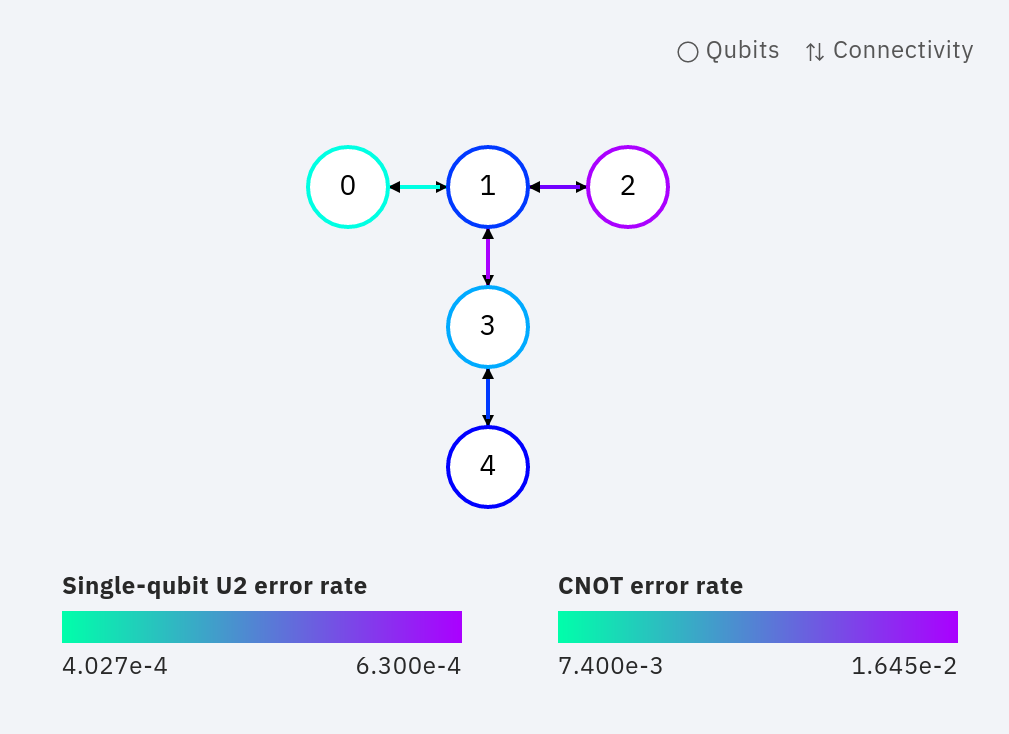
\includegraphics[width=0.48\textwidth]{images/connection_diagram_burlington.png}
\end{figure}

%%% Local Variables:
%%% mode: latex
%%% TeX-master: "report"
%%% End: